%%%%%%%%%%%%%%%%%%%%%%%%%%%%%%%%%%%%%%%%%%%%%%%%%%%%%%%%%%%%%%%%%%%%%%%%%%%%%
%%%
%%% File: thesis.tex, version 1.7, March 2021
%%%
%%% =============================================
%%% This file contains a template that can be used with the package
%%% cs.sty and LaTeX2e to produce a thesis that meets the requirements
%%% of the Computer Science Department from the Technical University of Cluj-Napoca
%%%%%%%%%%%%%%%%%%%%%%%%%%%%%%%%%%%%%%%%%%%%%%%%%%%%%%%%%%%%%%%%%%%%%%%%%%%%%

\documentclass[12pt,a4paper,twoside]{report}
\usepackage{cs}
\usepackage[T1]{fontenc}
\usepackage[utf8]{inputenc}
\usepackage[english]{babel}
\usepackage{times}
\usepackage{graphicx}
\usepackage{latexsym}
\usepackage{amsmath,amsbsy}
\usepackage{amssymb}
\usepackage[matrix,arrow]{xy}
\usepackage{ae,aecompl}
\usepackage{amstext}
\usepackage{graphics}
\usepackage{ae,aecompl}
\usepackage{algorithm}
\usepackage{color}
\usepackage{titlesec}
\usepackage{fancyhdr}
\usepackage{hyperref}
%% decomentati linia urmatoare pentru e nu mai evidenția hiper legăturile pentru imprimare pe hârtie
%\hypersetup{hidelinks}
\usepackage{geometry}
\usepackage{lipsum}
\usepackage{enumitem}

\setlist{noitemsep,nolistsep}

\diplomathesis
\centerchapter
\singlespace
\newenvironment{definition}[1][Definition.]{\begin{trivlist}
\item[\hskip \labelsep {\bfseries #1}]}{\end{trivlist}}

%%%%%%%%%%%%%%%%%%%%%%%%%%%%%% Change the last element accordingly
\renewcommand{\thesisauthor}{Z-Transformers}    %% Your first name(s) and family name.
\renewcommand{\thesismonth}{July}     %% The month of the licence session
\renewcommand{\thesisyear}{2024}      %% The year of the
\renewcommand{\thesistitle}{Bitbucket} % Title of the thesis
\renewcommand{\thesissupervisor}{Precup Alina, Ursu Denisa, Nealcos Mircea, Vanca Razvan} %% Supervisor
%%%%%%%%%%%%%%%%%%%%%%%%%%%%%%%%%%%%%
\newcommand{\makeThesisTitle}{\textbf{\thesistitletypesize \thesistitle}}
\newcommand{\makeThesisType}{\thesistypetypesize \thesistype}
\newcommand{\department}{\sffamily\bfseries\small FACULTY OF AUTOMATION AND COMPUTER SCIENCE}
\renewcommand{\thesistype}{Git solution for Jira}
\newcommand{\uline}[1]{\rule[0pt]{#1}{0.4pt}}
%\renewcommand{\thesisdedication}{Părinților mei}

% Headings pentru folie de capăt

 \geometry{
	a4paper,
	total={159.2mm,246.2mm},
	left=25.4mm,
	top=25.4mm,
}


\begin{document}
%\frontmatter
%%%%%%%%%%% Stil pentru paginile de capăt
\pagestyle{fancy}
\setlength{\voffset}{-10pt}
\setlength\headheight{70.0pt}
%\addtolength{\textheight}{-80.0pt}
\renewcommand{\headrulewidth}{0pt}
\chead{%
	
\includegraphics[width=\textwidth]{figs/AntetUTCNEng.pdf}
}
\cfoot{}
\lfoot{}
\rfoot{}
%\pagestyle{headings}
%%%%% Thesis title page %%%%%%%%%%%%%%%%%%%%%%%%
\begin{center}
	{\department}

	\vspace{4cm}
	\makeThesisTitle %LICENSE THESIS TITLE
	~\\~\\

	\makeThesisType

	~\\\vspace{6.5cm}

	\begin{tabular}{p{.3\linewidth}p{.5\linewidth}}
		{\hfill Team name:} & {\bf \thesisauthor} \\
		&\\
		{\parbox[t]{\linewidth}{\hfill Team members:}}& {\bf \thesissupervisor}\\
	\end{tabular}

	\vspace{3cm}
	{\bf \thesisyear}
\end{center}
%%%%%%%%%%%%%%%%% end of thesis title page %%%%%%%%%%%%%%%%%%%%%%%%%%%%%%%%%%%%
 % the first 3 pages
%%%%%%%%%%%%%%%%% Advices page to remove
\thispagestyle{empty}
\include{guideline}
\newpage
%%%%%%%%%%%%%%%%%% end of advices page
\pagestyle{fancy}
\setlength\headheight{16.0pt}
\renewcommand{\chaptermark}[1]{\markboth{\chaptername~\thechapter.~#1}{}}
\renewcommand{\sectionmark}[1]{\markright{\thesection\ #1}}
\renewcommand{\headrulewidth}{0.4pt}
\lhead{}
\chead{%
	\leftmark\rightmark
}
\chead{}
\cfoot{\thepage}
\lfoot{}
\rfoot{}

%%%%%%%%%%%% Table of contents
\pagenumbering{roman}
\setcounter{page}{1}

\newpage

\tableofcontents

\newpage

%\listoftables
%\listoffigures

\pagenumbering{arabic}
\setcounter{page}{1}


\titleformat{\chapter}[hang]
{\normalfont\Large\bfseries}{\chaptertitlename\ \thechapter.}{1em}{}
\titleformat{\section}[hang]
{\normalfont\large\bfseries}{\thesection.}{1em}{}
\titleformat{\subsection}[hang]
{\normalfont}{\thesubsection.}{1em}{}


\chapter{Introduction - Project Context}\label{ch:context}
\pagestyle{fancy}

{\color{blue}\noindent Should take 2 to three pages of the paper.\\}
\noindent What should be here:

\begin{itemize}
	\item framing the design theme in the contemporary context
	\item an outline of the exact domain of the design theme
\end{itemize}




 % \chapter{Introduction}

\chapter{Project Objectives}\label{ch:obiective}
\pagestyle{fancy}

{\noindent\color{blue}Should take 2 to 3 pages.\\}

Here you describe the design/research theme, precisely formulated, with clear objectives on 2-3 pages and, possibly, explanatory figures.


 % \chapter{Project Objectives}

\chapter{Bibliographic Research}\label{ch:studiubib}

\pagestyle{fancy}


{\color{blue}\noindent This chapter should take between 3 and 10 pages.\\}

Bibliographic research has as an objective the establishment of the references for the project, within the project domain/thematic. While writing this chapter (in general the whole document), the author will consider the knowledge accumulated from several dedicated disciplines in the second semester, 4$^{th}$ year (Project Elaboration Methodology, etc.), and other disciplines that are relevant to the project theme.

Each reference \textbf{must} be cited within the document. Please look at the examples below (depending on the project theme, the presentation of a method/application can vary).

Referințele are included in the Bibliography chapter.

References can by managed with \href{https://www.jabref.org/}{JabRef}, an application which can be downloaded from \url{https://www.jabref.org/#download}

Examples of what should be included in each type of reference can be found at \href{https://libguides.nps.edu/citation/ieee-bibtex}{here}.

About common errors found in online libraries of references you can read at \href{https://www.ece.ucdavis.edu/~jowens/biberrors.html}{here}


In Chapter 4 of ~\cite{Spizner2002}, Spitzner discusses the advantages and disadvantages of honeypot systems.

References will be included in the Bibliography section. The reference format must be IEEE, or similar. The introduction of new references in the Bibliography section, and their citation within the document text can be done manually (by obeying the format), but it is not recommended as it not easy to manage them, or by using the tools mentioned in the last paragraphs of this chapter.

In the Bibliography section, there are examples of references to conferences or workshops articles ~\cite{AntoniouSBB05}, journal ~\cite{AntoniouSBDB07}, and books ~\cite{russell1995artificial}, \cite{Spizner2002}. References to applications or online resources (web pages) must include at least a short relevant description in addition to the link~\cite{seleweb}, and other information is available (authors, year, etc.). References that contain only the link to the online resource will be placed in the page footer.

Each reference must be cited within the document text, see example below (depending
on the project theme, the presentation of a method/application can vary).

%În articolul~\cite{AntoniouSBDB07} autorii prezintă un sistem pentru ...
In paper~\cite{AntoniouSBDB07} the authors present a system for moving obstacle detection using stereo-vision and an estimation of own movement.

The method is based on ... autorii prezintă un sistem pentru detecția obstacolelor în mișcare folosind stereo viziune și estimarea mișcării proprii.
Metoda se bazează pe ...\textit{discuss the algorithms, data structures, functionality, specific aspects related to the project theme, etc….} Discussion: \textit{pros and cons}.

\section{A Section Name}
\section{Another Section Name}
\subsection{A Subsection Name}
{\color{red}DO NOT copy technology descriptions here}

 % \chapter{Bibliographic Research}

\chapter{Analysis and Theoretical Foundation}
\label{ch:analysis}
\pagestyle{fancy}

{\color{blue}Together with the next two chapters takes about 70\% of the whole paper.\\}

The purpose of this chapter is to explain the operating principles of the implemented
application.
Here you write about your solution from a theory standpoint – i.e. you explain it and demonstrate its theoretical properties/value, e.g.:
\begin{itemize}
	\item used or proposed algorithms,
    \item used protocols,
    \item  abstract models,
    \item  logic explanations/arguments concerning the chosen solution,
    \item  logic and functional structure of the application, etc.
\end{itemize}


~\\\parbox[c]{\textwidth}{\color{red}\bfseries

YOU SHOULD NOT write about the implementation.
YOU SHOULD NOT describe technologies and other things which do not pertain to
your project (no fillers, please!).
}


\section{A section title}\label{sec:context}

\subsection{A Subsection title}

Every table in the thesis should be numbered as Table \textit{x.y}, where \textit{x} is the chapter number where the table is included, and \textit{y} is the number of the table within that chapter. There should be one empty line after the paragraph preceding the table, and one empty line after the table. Example: in this row we have inserted a reference to Table~\ref{tab:nonlin}.

\begin{table}[ht]
    \caption{Results} % table caption
    \label{tab:nonlin} % \label{table:nonlin} introduces the label used to refer the table in the textt; reference is achieved via \ref{table:nonlin}
    \centering                          % centered table
    \begin{tabular}{|c|c|c|c|}          % 4 centerered columns
        \hline
        Case & Method\#1 & Method\#2 & Method\#3 \\ [0.5ex]   % heading
        \hline                              % single horizontal line
        1 & 50 & 837 & 970 \\               % table body
        2 & 47 & 877 & 230 \\
        3 & 31 & 25 & 415 \\[1ex]           % [1ex] adds vertical space
        \hline
    \end{tabular}

\end{table}

Every figure used in the thesis should be referred  (e.g. Figure x.y shows the components of the system...) and numbered.

Numbering is like this: Figure \textit{x.y} where \textit{x} is the chapter number and \textit{y} is the number of the figure within that chapter. E.g. , in this row we have inserted a reference to Figure~\ref{fig:imag}.

\begin{figure}[ht]
    \centering
    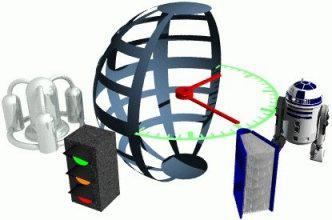
\includegraphics[]{figs/test.jpg}
    \caption{Figure name}
    \label{fig:imag}
\end{figure}

 % \chapter{ Analysis and Theoretical Foundation}

\chapter{Detailed Design and Implementation}
\pagestyle{fancy}

{\color{blue}Together with the previous and next chapter takes about 70\% of the paper.\\}


The purpose of this chapter is to document the developed application such a way that it
can be maintained and developed later. A reader should be able (from what you have written
here) to identify the main functions of the application.

The chapter should contain (but not limited to):
\begin{itemize}
	\item  a general application sketch/scheme,
    \item  a description of every component implemented, at module level,
    \item  class diagrams, important classes and methods from key classes.
\end{itemize}

 % \chapter{Detailed Design and Implementation}

\chapter{Testing and Validation}
\pagestyle{fancy}

{\noindent\color{blue}Together with the previous two chapters should take about 70\% of the paper.}

 % \chapter{Testing and Validation}

\chapter{User’s Manual}
\pagestyle{fancy}

In the section describing the installation procedure you should detail the hardware and
software resources needed for installing and running the application, and a step by step
description of how your application can be deployed/installed. An administrator should be able
to perform the installation/deployment based on your instructions.


In the section for the user you should describe how to use the application from the point
of view of a user with no inside technical information; this should be adorned with screen shots
and a stepwise explanation of the interaction. Based on user's manual, a person should be able
to install and use your product.

{\noindent\color{blue}Should take 1 to 5 pages.\\}
 % \chapter{User’s manual}

\chapter{Conclusions}
\pagestyle{fancy}

{\color{blue} This chapter should take one or two pages.\\}

In this chapter you should include::
\begin{itemize}
	\item A summary of your contributions/achievements,
    \item  A critical analysis of the results achieved,
    \item  A description of the possibilities of improvements/further development.
\end{itemize}

 % \chapter{Concluzii}


\bibliographystyle{IEEEtran}
\bibliography{thesis}%same file name as for .bib

\appendix
\chapter{Relevant Code sections}
\pagestyle{fancy}

\begin{verbatim}
 /** Maps are easy to use in Scala. */
object Maps {
  val colors = Map("red" -> 0xFF0000,
                   "turquoise" -> 0x00FFFF,
                   "black" -> 0x000000,
                   "orange" -> 0xFF8040,
                   "brown" -> 0x804000)
  def main(args: Array[String]) {
    for (name <- args) println(
      colors.get(name) match {
        case Some(code) =>
          name + " has code: " + code
        case None =>
          "Unknown color: " + name
      }
    )
  }
}
\end{verbatim}

\chapter{Other Relevant Info}

Proofs etc. if any. Otherwise remove this chapter

\chapter{Published Papers}

If any. Otherwise remove this chapter

\end{document}
